\documentclass{article}
\usepackage{amsmath}
\usepackage{float}
\usepackage{graphicx}
\title{The Magellanic Stream}
\author{Xin Gao}
\date{}
\begin{document}
\maketitle

\section{Abstract}
\section{Introduction}
The Magellanic Clouds are satellite galaxies of the Milky Way in the
southern direction relative to the Milky Way's galactic plane at about
50 kiloparsecs away. They are large cloud structures home to regions of
rapid star formation. A very large stream of dust cloud stretching
between the Magellanic Clouds and stretching far away from the end of
the Small Magellanic Cloud was discovered  about half a century ago. It
spans nearly 180 degrees in the sky from the view of the Earth. Using
the Leuschner Dish, we receive radio signals from the stream. We then 
replicate a 2-D image of the stream with those signals by applying image
processing and staistical techniques. Ultimately, the product reflects
reality in galactic space, using galactic coordinates with a velocity
dimension to indicate relative depth.
\section{Methods and Procedure}
It is particularly convenient for radio astronomy to study
cosmic-scale objects due to the universality of the photons
corresponding to the energy release of the hydrogen hyperfine
transition. The physics of this study is centered on astrophysical
techniques for interpretating the data sets collected by the dish at the
hyperfine hydrogen line and how to manipulate the data sets to
extrapolate information that would be used to image the source.  
\subsection{Galactic Coordinates and the Local Group}
While equatorial coordinates are useful for assigning stellar locations
on the intra-galactic scale, galactic coordinates for convenient for
mapping Local Group objects on the inter-galactic scale, which consists
of the Milky Way, the Andromeda, and the Triangulum galaxies with many
surrounding dwarf and satellite galaxies. At the origin of the galactic
coordinate system is the Sun. The galactic longitude (l) begins
counterclockwise in the direction towards the galactic center. The
latitude (b) is centered on the galactic plane. For example, the Large
Magellanic Cloud during the J2000 epoch has equatorial coordinates of
$(ra=80.894^{\circ} , dec=-69.756^{\circ})$ with a corresponding
galactic coordinates of $(l=280.465^{\circ} , b=-32.889^{\circ})$. The
coordinates can be changed from equatorial to galactic through an
epoch-dependent rotation matrix; for the J2000 era, it is:
\begin{align}R_{(ra,dec)\rightarrow(l,b)} = \begin{pmatrix}-0.054876 &
    -0.873437 & -0.483835 \\ 0.494109 & -.0444830 & 0.746982 \\
    -0.867666 & -0.198076 & 0.455984\end{pmatrix}
\end{align}
The goal here is to map the Magellanic Stream in 3-D coordinates of
(l,b,v) where v is relative velocity, which indicates depth and other
regional variations.
\subsection{The 21-cm Hyperfine Transition Line of Hydrogen}
\subsection{Emission and Absorption Lines from Distant Sources}
\subsubsection{Broadening}
\subsubsection{The Line Profile Function}
\subsection{Intensity Calibration}
In order to produce meaningful data for mapping, we calibrate the
intensity of our data to produce temperature spectra that can show the
variations among the values of our data. The calibration is done through
the following equation:
\begin{align}T_{sys} + T(\nu) =
  \Big[\frac{P_j^{Online,CalOff}}{P_{j}^{Offline,CalOff}}\Big]
  \Big[\frac{\sum_{j=0}^{2J-1}P_{j}^{Offline,CalOff}}
  {\sum_{j=0}^{2J-1}(P_{j}^{Offline,CalOn} - P_{j}^{Offline,CalOff})}\Big]T_{Cal} 
\end{align}
$T_{sys}$ is the frequency independent portion of the total system
temperature. It comes from the electronics in our tools and the
interference of sources, such as the Earth's atmosphere and the galaxy's
synchrotron radiation, other than our target. $T(\nu)$ is the frequency
dependent temperature and is what we would want as the data from our
source. P is power and j denotes a specific frequency with J being the
total number of discrete frequencies in our data. Offline and Online
denote the status of our oscillator; CalOff and CalOn denote the status
of the presence of the noise, whose corresponding temperature is
$T_{Cal}$. 
\section{Data}
Data were taken in ranges of $58^{\circ}$ to $90^{\circ}$ in longitude and
$60^{\circ}$ to $82^{\circ}$ in latitude. Each set of coordinates
corresponds to several pointings of 358 average (of the Local Oscillator
on and off) samples per pointing. Each pointing consists of four sets of
array data varying among the on or off status of the local oscillator
and of the noise data array. The initial data shows the power received
as a function of frequency. The following shows the data set for a
pointing.
\begin{figure}[h]
\centering
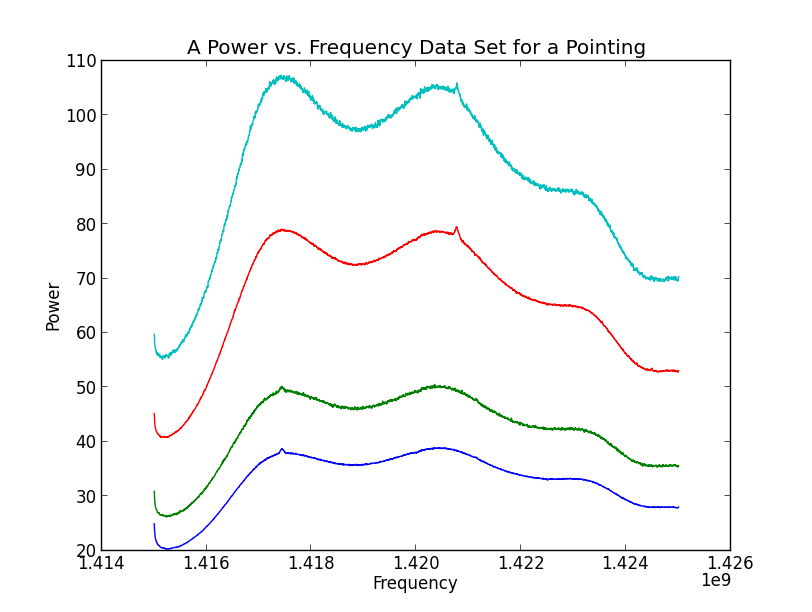
\includegraphics[width=.9\textwidth]{point_data.png}
\caption{Plots showing data for a pointing at the
  $(66.0^{\circ},-72.0^{\circ})$ coordinate. From the lowest power to
  highest power curves: oscillator on and noise off; oscillator and
  noise on; oscillator and noise off; oscillator off and noise on.} 
\end{figure}
All data sets received are similar in shape, but differ in subtleties
and the location of the 'spike.'
\section{Analysis}
We apply the calibration method described above to the data from the
$58^{\circ}$ to $90^{\circ}$ pointing. $T_{Cal}$ is about 100 K. The first
bracket in the calibration equation suggests that that ratio is
frequency dependent, so we are free to choose any pair of corresponding
points for that calculation refers to the shape of the data; it is a
ratio of the online array to the offline array. The second bracket is
the holistic frequency independent system temperature, taking into
account the entire range of frequencies. 
\section{Conclusion}

\end{document}
